RIS, which consists of an array of passive reflecting elements, is attracting many researchers and 
is regarded as a promising technique for NG wireless communications \cite{liu2020RIS}. Due to its capability of intelligently 
reconfiguring the gain and phase of the signal, it can adjust the propagation environment for a wireless communication system
and make improvements in terms of required power, achievable rate, SINR, etc.

\subsection{System Model}

Figure \ref{fig:ris-aided-wireless-system} depicts an example of a RIS-assisted wireless communication system.

\begin{figure}[htbp]
    \centering
    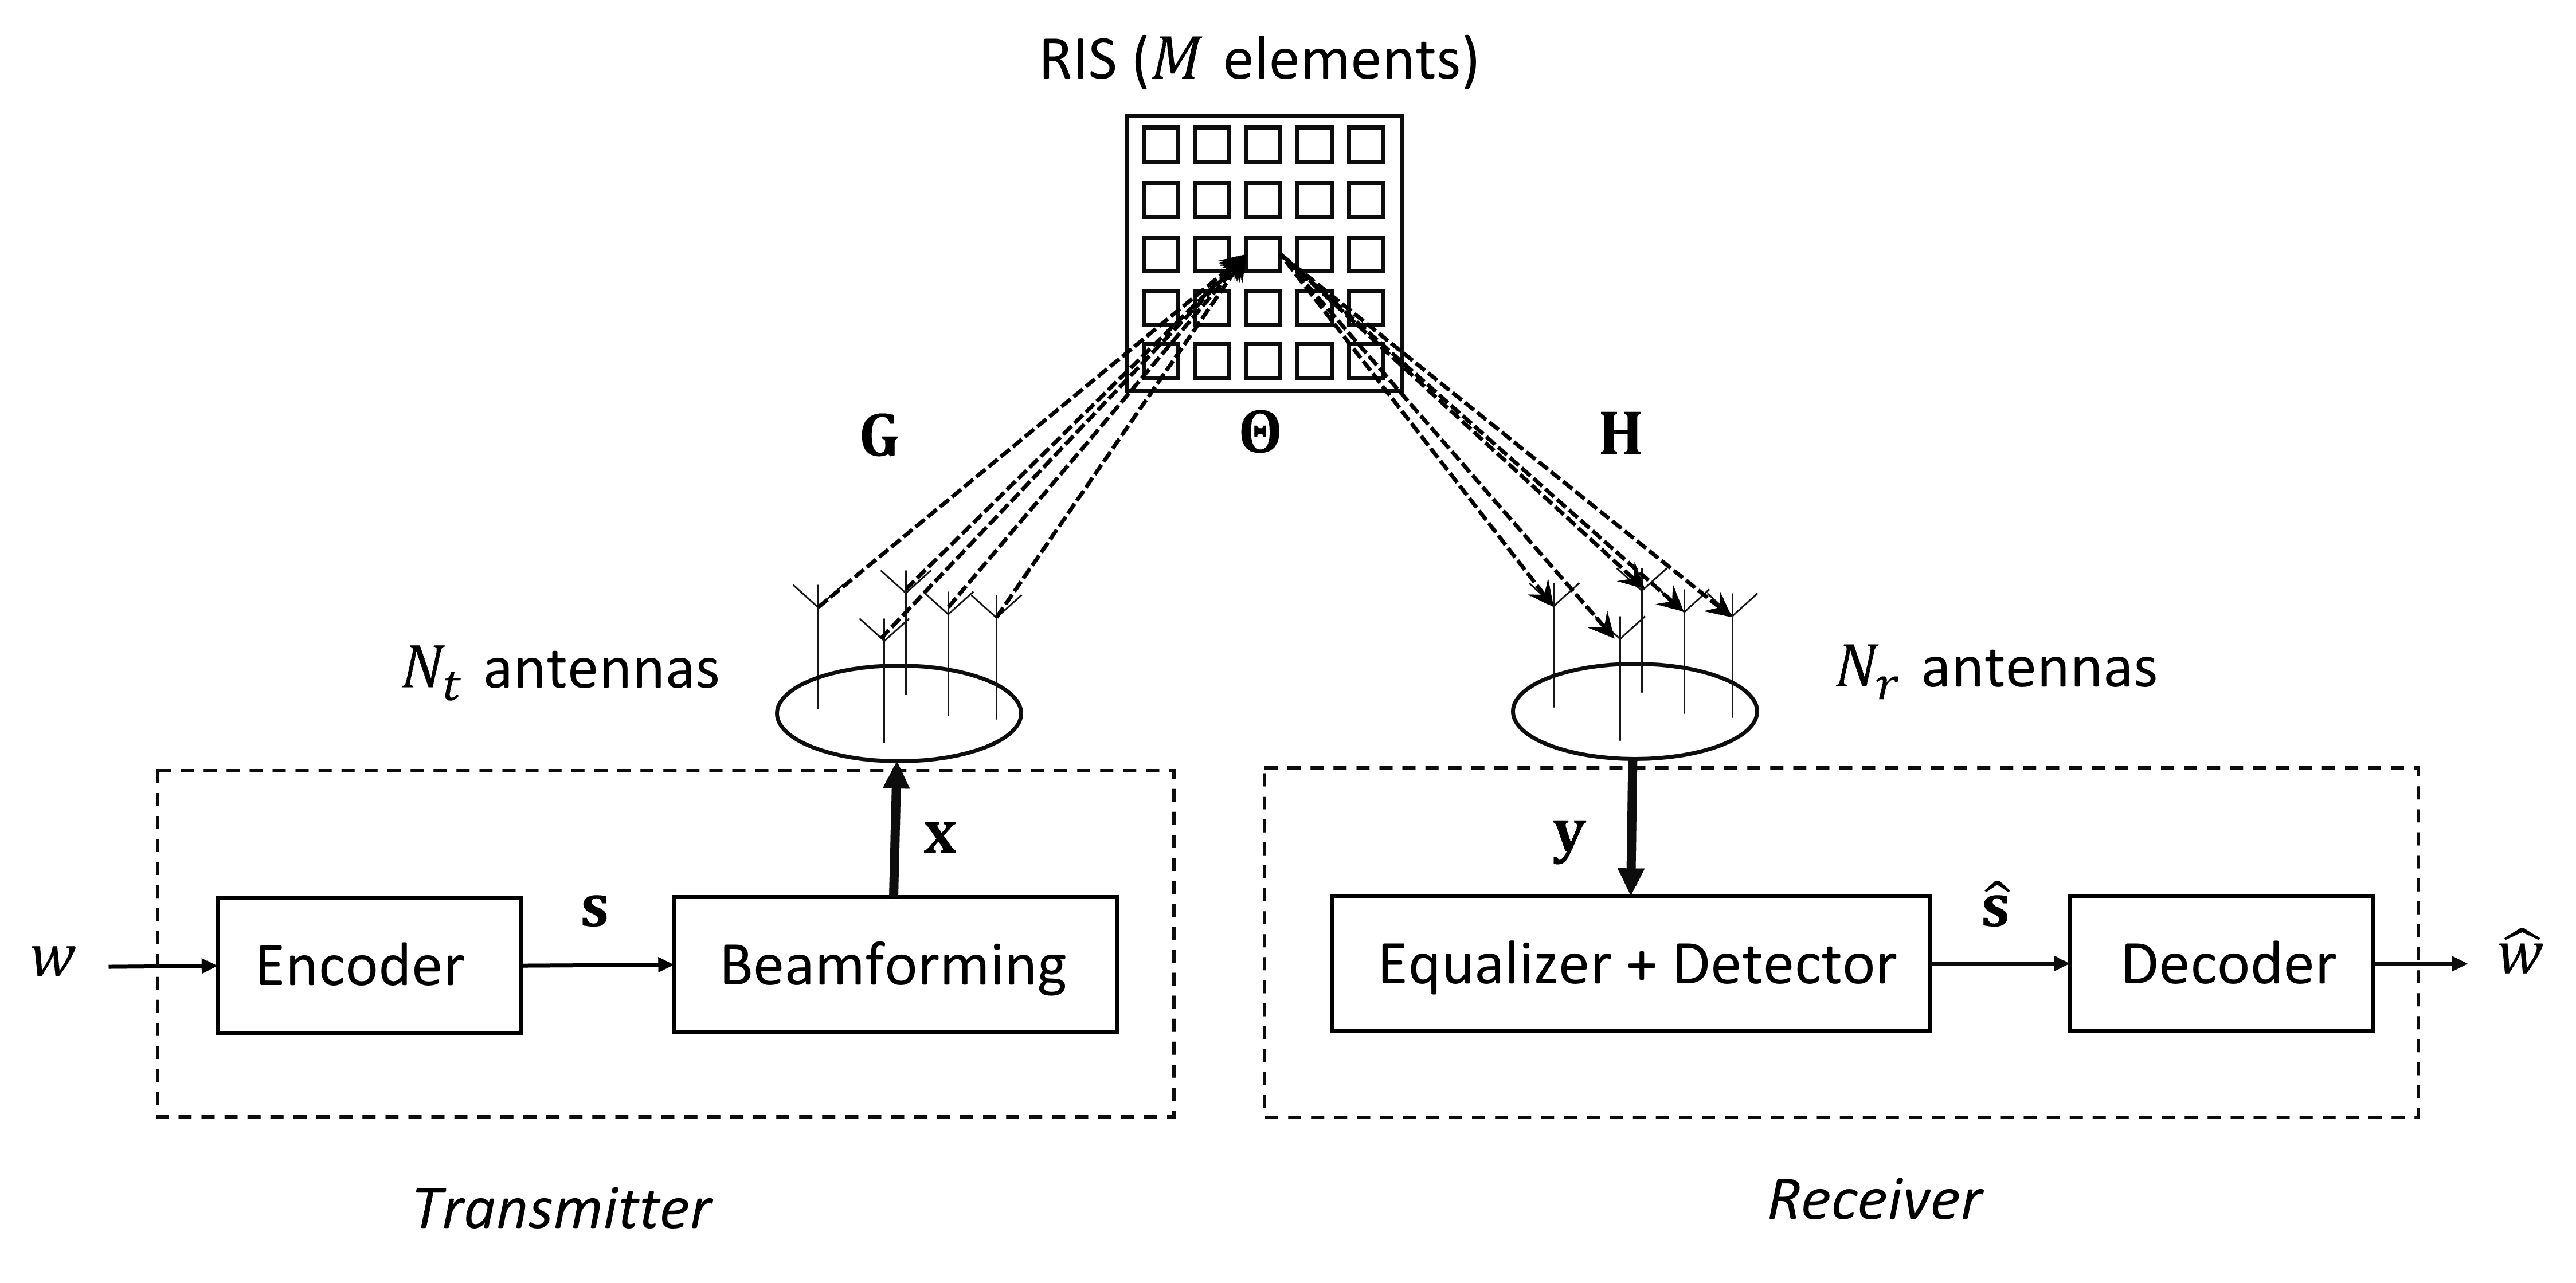
\includegraphics[width=1.0\textwidth]{./ris-aided-wireless-system.png}
    \caption{RIS-aided wireless communication system}
    \label{fig:ris-aided-wireless-system}
\end{figure}

Through the RIS-adied channel, the received signal is given as
\begin{equation} \label{eqn:ris-signal-model}
    {\bf y} = {\bf H\Theta Gx + n} = {\bf H\Theta GPs +n} = \underbrace{\bf H\Theta G}_{{\bf \tilde{\bf H}}}\sum_{i=1}^R {\bf p}_i s_i + {\bf n},
\end{equation}
where ${\bf G} \in \mathbb{C}^{N_t \times M}$ denotes the channel between transmitter and RIS 
and ${\bf H} \in \mathbb{C}^{M \times N_r}$ denotes the channel between RIS and receiver.
${\bf \Theta} \in \mathbb{C}^{M \times M}$ is the reflecting matrix of RIS.
Compared with \eqref{eqn:wireless-received-signal-beamforming}, we can see that the efficient channel $\tilde{\bf H} = {\bf H\Theta G}$ 
in RIS-aided system can be adjusted by optimizing ${\bf \Theta}$, which is called passive beamforming. Generally, the 
active beamforming ${\bf P}$ and passive beamforming ${\bf \Theta}$ are jointly designed to maximize or minimize some 
communication metrics.

Now we consider an achievable rate maximization problem. For a MIMO system, the achievable rate is given as
\begin{equation}
    R = \log_2 \det \left( {\bf I}_{N_r} + \frac{1}{\sigma_n^2} \tilde{\bf H} {\bf P}{\bf P}^H \tilde{\bf H} \right).
\end{equation}
Thus, the problem of maximising the achievable rate can be phrased as
\begin{subequations} \label{problem:ris-rate-example}
    \begin{align}
      \max_{{\bf P, \Theta}} \quad &R({\bf P, \Theta}) \\
      \mathrm{s.t.} \quad & \mathrm{Tr}({\bf PP}^H) \leq P_t, \\ 
      & {\bf \Theta} \in \mathcal{Q},
    \end{align}
\end{subequations}
where the first constraint stands for the power budget. $\mathcal{Q}$ denotes the feasible set of reflecting matrix ${\bf \Theta}$,
which will be discussed in the next section.

\subsection{Reconfigurable Intelligent Surface Model}
In most literature, the RIS is modeled that each reflecting element works independently. Figure \ref{fig:conventional_RIS_model}
shows the hardware model of RIS. Each element can be realized by a varactor diode, the equivalent load impedance of which can be adjusted by changing bias voltage \cite{liu2020RIS}.
In theory, each element can be characterized by the reflection coefficient
\begin{equation}
    r = \beta e^{j \phi},
\end{equation} 
where $\beta \in [0,1]$ controls the gain and $\phi \in [0,2\pi]$ controls the phase shift of reflected signal.

\begin{figure}[htbp]
    \centering
    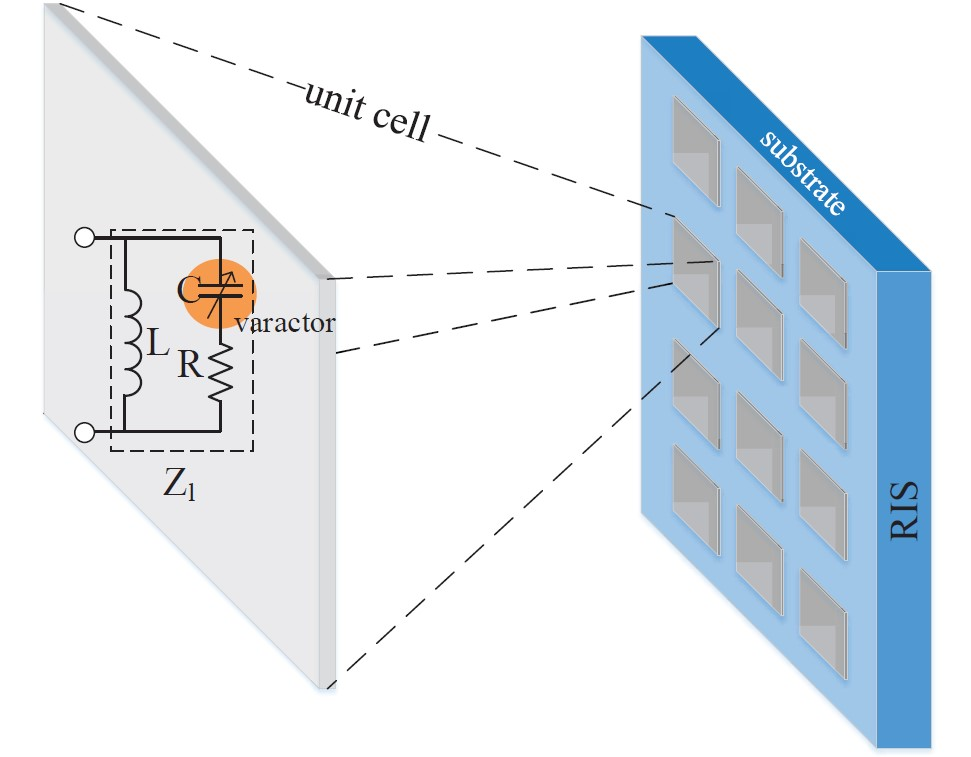
\includegraphics[width=0.6\textwidth]{./conventional_RIS_model.jpg}
    \caption{Hardware model of RIS \cite{liu2020RIS}}
    \label{fig:conventional_RIS_model}
\end{figure}

As each element works independently in this model, the reflecting matrix ${\bf \Theta}$ in \eqref{eqn:ris-signal-model} is a diagonal matrix:
\begin{equation}
    {\bf \Theta} = \mathrm{diag}\left( \beta_1 e^{\phi_1},\beta_2 e^{\phi_2},...,\beta_M e^{\phi_M} \right),
\end{equation}
In this case, by letting $\theta_i = \beta_i e^{j\phi_i}$, the problem \eqref{problem:ris-rate-example} can be written as
\begin{subequations}
    \begin{align}
      \max_{{\bf P, \Theta}} \quad &R({\bf P, \Theta}) \\
      \mathrm{s.t.} \quad & \mathrm{Tr}({\bf PP}^H) \leq P_t, \\ 
      & {\bf \Theta} = \mathrm{diag}\left( \theta_1,\theta_2,...,\theta_M \right),\\
      & |\theta_i| \leq 1, \forall i.
    \end{align}
\end{subequations}

Recently, Shen el al. \cite{shen2020modeling} proposed a novel RIS model (Figure \ref{fig:single_fully_RIS} and \ref{fig:group_RIS}) base on scattering parameter network analysis. In this
novel model, the elements of RIS are group or fully connected instead of working independently, which shows advantages 
on received power in Rayleigh channel. The constraints of group and fully connected RIS model are given as
\begin{enumerate}
    \item Grouped connected: ${\bf \Theta} = \mathrm{diag}({\bf \Theta}_1,{\bf \Theta}_2,...,{\bf \Theta}_G), {\bf \Theta}_g={\bf \Theta}_g^T,{\bf \Theta}_g^H {\bf \Theta}_g \preceq {\bf I},\forall g$;
    \item Fully connected: ${\bf \Theta} = {\bf \Theta}^T, {\bf \Theta}^H {\bf \Theta} \preceq {\bf I}$.
\end{enumerate}

When the number of group $G$ equals to $1$, group connected RIS is equivalent to fully connected RIS; when 
$G$ equals to the elements number $M$, group connected RIS is equivalent to single connected RIS, i.e., each element works independently.

\begin{figure}[htbp]
    \centering
    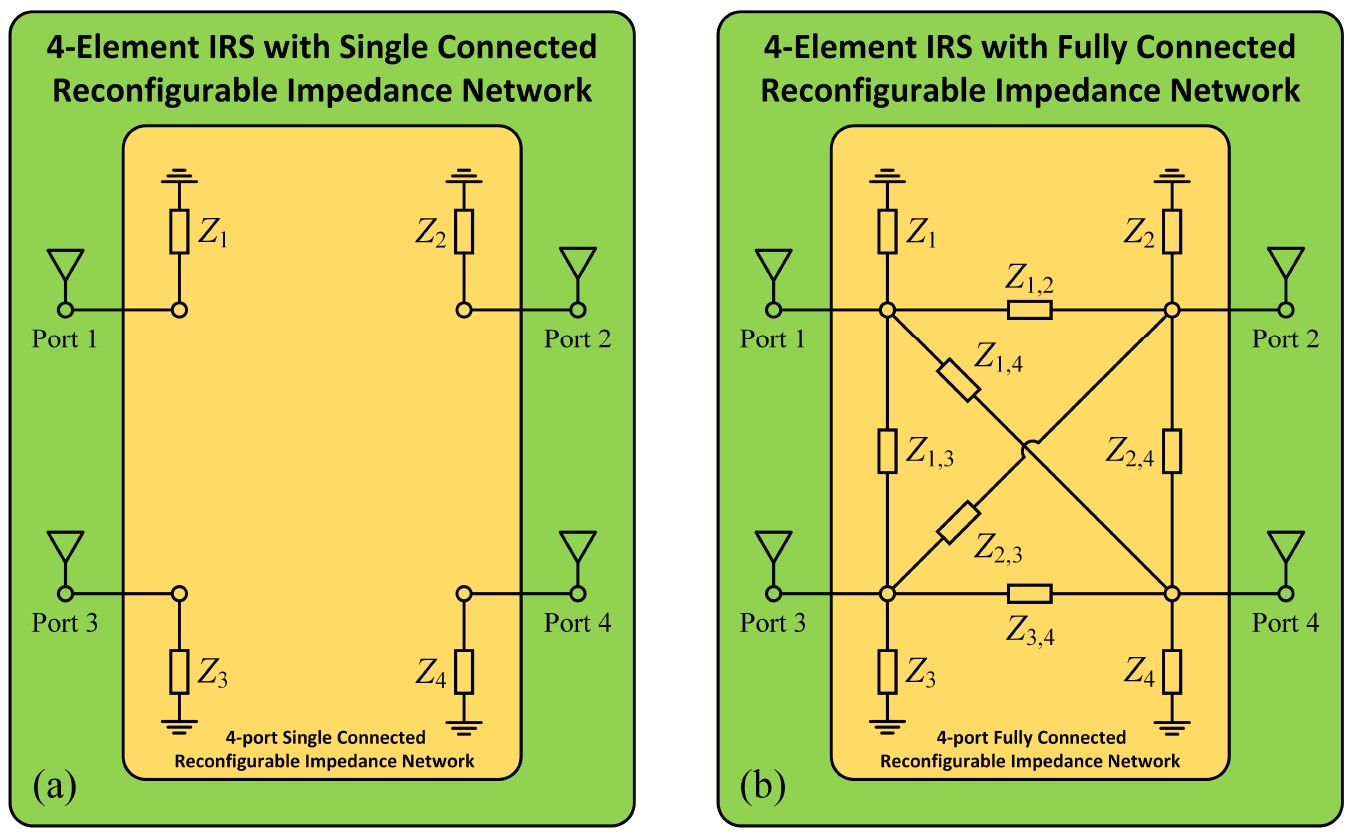
\includegraphics[width=0.6\textwidth]{./single_fully_RIS.jpg}
    \caption{Model of single (a) and fully (b) connected RIS \cite{shen2020modeling}}
    \label{fig:single_fully_RIS}
\end{figure}

\begin{figure}[htbp]
    \centering
    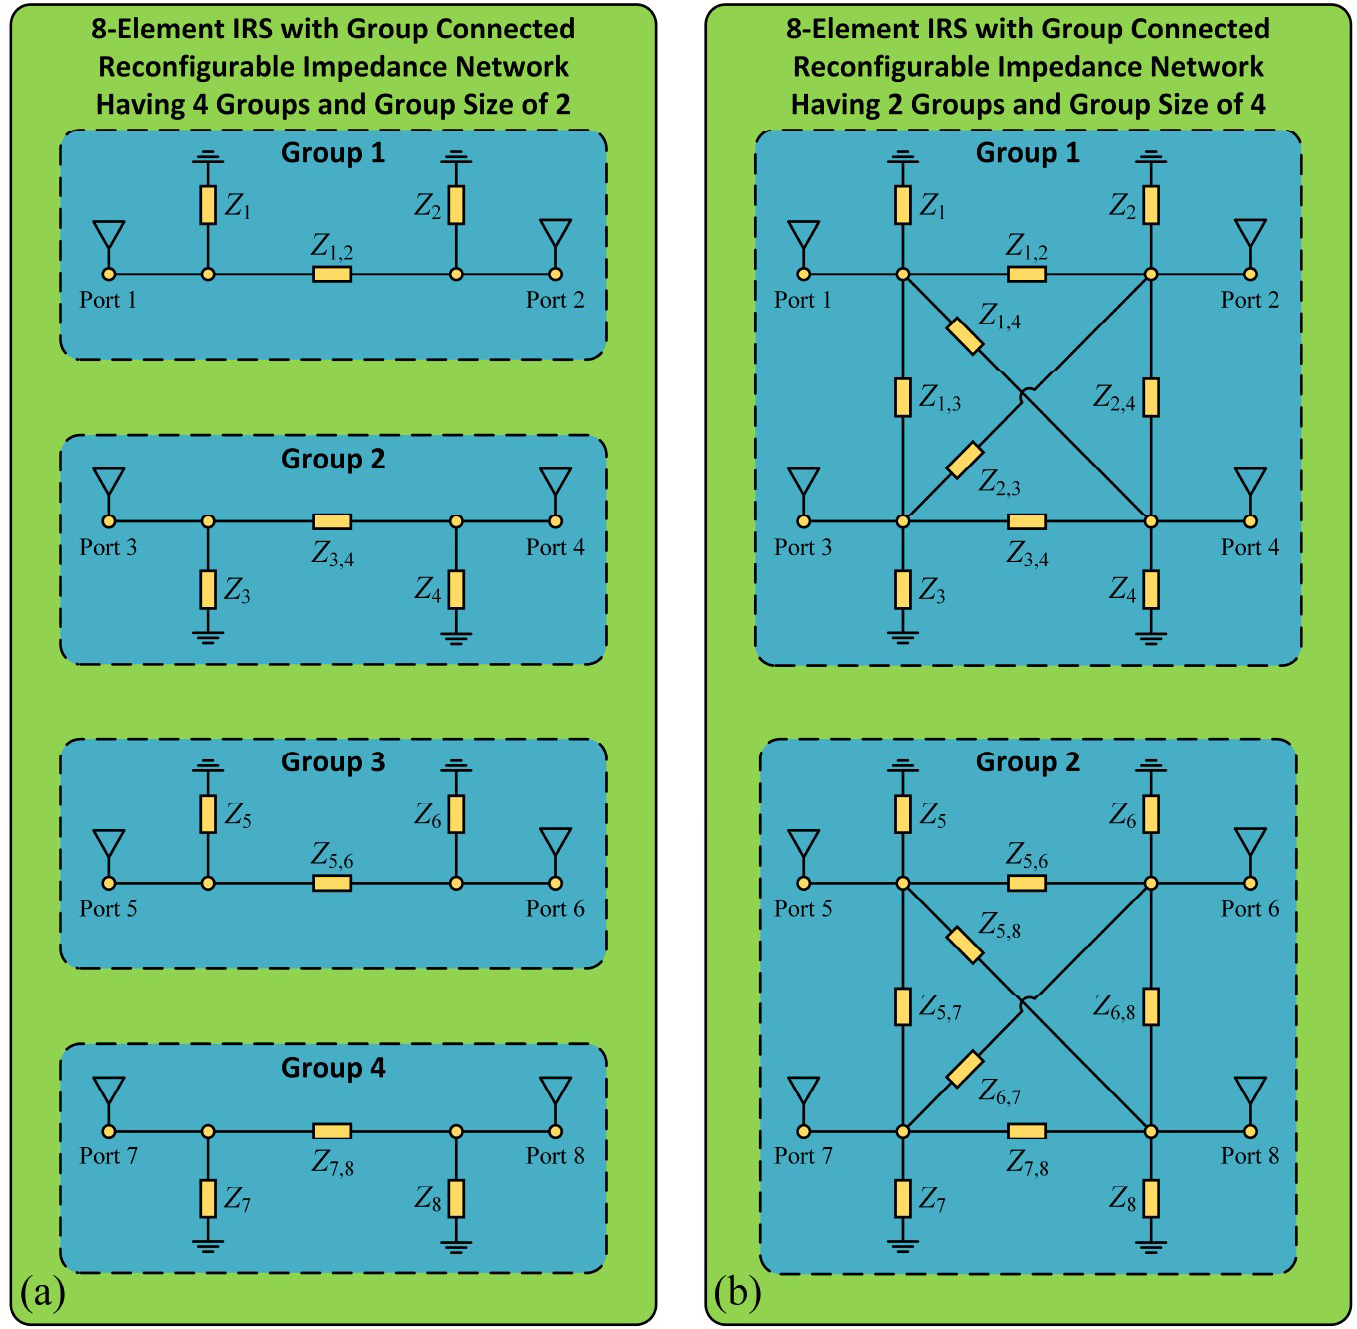
\includegraphics[width=0.6\textwidth]{./group_RIS.jpg}
    \caption{Model of group connected RIS\cite{shen2020modeling}}
    \label{fig:group_RIS}
\end{figure}